%%%%%%%%%%%%LASCIARE QUESTI COMMENTI!!!%%%%%%%%%%%%%%%%
% !TeX document-id = {02478c5b-a4cd-4f4c-a426-82311f1967ba}
% !TeX TXS-program:compile = txs:///pdflatex/[--shell-escape]
%%%%%%%%%%%%%%%%%%%%%%%%%%%%%%%%%%%%%%%%%%%%%

\documentclass[10pt,hidelinks]{article}
\usepackage[utf8]{inputenc}
\usepackage[british]{babel}
\usepackage{mdframed}

%%MUST STAY HERE
\usepackage[svgnames, table]{xcolor}
%%

\usepackage{algorithm}
\usepackage{algpseudocode}
\usepackage{amsfonts}
\usepackage{amsthm}
\usepackage{amsmath}
\usepackage{array}
\usepackage{amssymb}
\usepackage{arydshln}

\usepackage{bbding}
\usepackage{booktabs}

\usepackage[colorlinks = true,
            linkcolor = pdarkerblue,
            urlcolor  = gblue,
            citecolor = gblue,
            anchorcolor = blue]{hyperref}%%Must stay here
%%

\usepackage{calc}
\usepackage[labelfont={bf,sf,footnotesize,color=pblue},textfont={footnotesize}, margin={40pt,40pt}]{caption}
\usepackage{cleveref}
\usepackage{csquotes}
\usepackage{dsfont}

\usepackage{enumitem}
\usepackage{eurosym}

\usepackage{fancyhdr}
\pagestyle{fancy}
\fancyhead{}
\fancyhead[R]{\color{pblue} \sc \nomefico}
\lhead{\includegraphics[width=1cm]{pics/Cherubino.jpg}}
\usepackage[T1]{fontenc}
\usepackage{fullpage}

\usepackage{geometry}

\usepackage{graphicx}

\usepackage{hhline}
\usepackage{listings}
\usepackage{lipsum}

\usepackage{mathrsfs}
\usepackage{mathtools}
\usepackage{minted}
\usepackage{multicol}
\usepackage{multirow}

\usepackage[numbers,sort]{natbib}
\usepackage{navigator}

\usepackage{palatino}
\usepackage{pifont}
\usepackage{pgffor}
\usepackage{pgfplots}
\usepackage{pgfplotstable}
\usepackage{placeins}

%\usepackage{showframe}
\usepackage{sectsty}
\usepackage{siunitx}
%\usepackage{subfig}
\usepackage{subcaption}

\usepackage{tabularx}
\usepackage[many]{tcolorbox}
\usepackage{tikz}
\usepackage{todonotes}

\usepackage{verbatim}

\usepackage{wrapfig}

\usepackage{xinttools}

%%%~~~~~~~~~~~~~~~~~~~~~~~~Fonts~~~~~~~~~~~~~~~~~~~~~~~%%%


%%%~~~~~~~~~~~~~~~~~~~~~~~~Colours~~~~~~~~~~~~~~~~~~~~~%%%
\definecolor{gblue}{HTML}{000099}
\definecolor{pblue}{HTML}{00004d}%{0000FF}
\definecolor{pdarkblue}{HTML}{000080}
\definecolor{pdarkerblue}{HTML}{000066}
%\definecolor{veryblue}{HTML}{00004d}

%~~~~~~~~~~~~~~~~~~~~~~~~~~~~~Tikz~~~~~~~~~~~~~~~~~~~~~~~~~~~~~%
\usetikzlibrary{calc}
\usetikzlibrary{shapes,arrows,arrows.meta}
\usetikzlibrary{automata,positioning}
\usetikzlibrary{spy,backgrounds}
\usetikzlibrary{matrix,positioning,arrows.meta,arrows}
\usetikzlibrary{fadings}
\usetikzlibrary{positioning}
\usetikzlibrary{fit}

\newcommand\nomefico{\textbf{Sapientino}}
\newcommand{\R}{\mathds{R}}


\pgfplotsset{compat=1.15}

\sectionfont{\bf \Large \color{pblue}}
\subsectionfont{\bf \color{pdarkblue}}
\subsubsectionfont{\bf \color{pdarkerblue}}

\mdfdefinestyle{MyFrame}{%
    linecolor=pdarkblue,
    fontcolor=white,
    outerlinewidth=2pt,
    roundcorner=20pt,
    innertopmargin=4pt,
    innerbottommargin=4pt,
    innerrightmargin=4pt,
    innerleftmargin=4pt,
    leftmargin = 4pt,
    rightmargin = 4pt,
    backgroundcolor=pdarkerblue
}

 \renewcommand{\labelitemi}{$\textcolor{pblue}{\diamond}$}

\DeclareMathOperator*{\avg}{avg}


\def\colOne{white}
\def\colTwo{pblue!10}
\def\colHea{pblue!35}


%%%%%%%%%%%%%%%%%%%%%%%%%%%%%%%%%%%%%%%%%%%%%%%%%%%%%%%%%%%%%%%%%%%%%%%%%%%%%%%%%%

\begin{document}

\begin{titlepage}
    \centering
    \scalebox{0.8} {
        \begin{minipage}{0.22\textwidth}%
            \includegraphics[width=\linewidth]{pics/Cherubino.jpg}
        \end{minipage}\hspace{10pt}
        \begin{minipage}{0.9\textwidth}%
            \flushright
            \large
            \vspace{0.8cm}
            \textsc{\color{pblue}%
            \nomefico\\
            a Bert-based, open domain\\
            question answering system}
            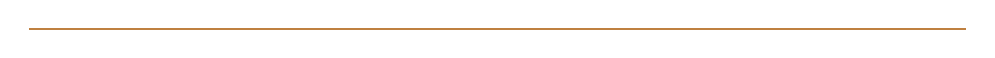
\begin{tikzpicture}%
                \draw[thick, brown] (0.1,0)--(0.99\textwidth,0);%   
            \end{tikzpicture}%
        \end{minipage}%
    }

    \vspace{0.3cm}
    
    Gabriele Barreca, Mario Bonsembiante {\small and} Gemma Martini
    
    %\vspace{0.4cm}
    
    {\scriptsize University of Pisa}
    
    \vspace{0.7cm}
    
    \abstract{
        \footnotesize
        Question answering (QA) systems can be seen as information retrieval systems which aim is to respond to queries, stated in natural language, by returning short answers or long sentences.
        The ``so-called'' \emph{open domain QA task} adds the challenge of understanding if the answer to the selected question may or may not be found in a given paragraph, which content has been buried within large text corpora, such as Wikipedia.
    
        \vspace{0.1cm}
    
        Building such systems for practical applications has historically been quite challenging and involved.
        The spectrum of possible answers given a question and a paragraph, moves from the ``simple'' \emph{yes/no answers} to the longer and more articulated \emph{long answers}, to then get to a trade-off between expressive power and succinctness, the ``so-called'' \emph{short answers}, which aim to enclose the answer in a single and possibly short sentence.
        
        \vspace{0.1cm}
        
        In this paper, we present a BERT-based implementation that solves an open domain QA task, providing all the three categories of answers listed above, with particular attention on the most widely studied kind, i.e.~short answers.
        We achieve pretty good results, although not as good as the state-of-the-art, that was not the purpose of this work.
        
        \vspace{0.1cm}
        
        As expected and already stated in previous work, we conclude that predicting long answers per se is pretty unreliable, while much better results are achieved if the short answer is predicted and then enlarged with the whole paragraph it lies in, from the original text.
    }

    
    \vspace{1cm}
    
    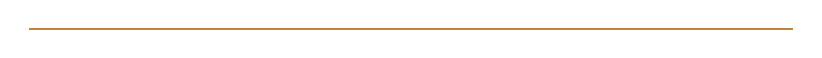
\begin{tikzpicture}%
        \draw[thick, brown] (0,0)--(0.8\textwidth,0);%   
    \end{tikzpicture}%
    
    %\vspace{-0.5cm}
    \scalebox{0.8}{\vbox{\large \tableofcontents}}
    %\tableofcontents

    \vspace{0.1cm}

    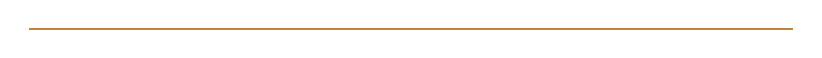
\begin{tikzpicture}%    
        \draw[thick, brown] (0,0)--(0.8\textwidth,0);%   
    \end{tikzpicture}%

    %{\large \today}
    \vfill
\end{titlepage}

%%%%%%%%%%%%%%%%%%%%%%%%%%%%%%%%%%%%%%%%%%%%%%%%%%%%%%%%%%%%%%%%%%

%\thispagestyle{empty}
\newpage
\newgeometry{
	right=45mm,
	left=40mm,
	top=40mm,
	bottom=45mm
}
\setcounter{page}{1}

%%%%%%%%%%%%%%%%%%%%%%%%%%%%%%%%%%%%%%%%%%%%%%%%%%%%%%%%%%%%%%%%%%
\section{Introduction}\label{sec:intro}
%%%%%%%%%%%%%%%%%%%%%%%%%%%%%%%%%%%%%%%%%%%%%%%%%%%%%%%%%%%%%%%%%%

In this paper we present \nomefico, a full pipeline for answering to open domain questions.
We developed in Flask an API for answering general open domain questions.
We then built a website and an app that utilizes this API for answering user defined, open domain questions.
By means of our platform, any user can ask questions and \nomefico~uses Wikipedia pages and our BERT-based model for answering these questions. 
This API is easily transferable to new implementations, e.g. a vocal assistant.

This report is structured as follows: in \Cref{sec:architecture}, the overall architecture is described and then (\Cref{sec:dataset}) we dig into the details of the choice of NQ dataset. In \Cref{sec:model} we explain the architecture of \nomefico, followed by a study of the performances and a mention (\Cref{sec:conclusions_and_future_work}) to what is yet to come.

%%%%%%%%%%%%%%%%%%%%%%%%%%%%%%%%%%%%%%%%%%%%%%%%%%%%%%%%%%%%%%%%%%
\section{The architecture}\label{sec:architecture}
%%%%%%%%%%%%%%%%%%%%%%%%%%%%%%%%%%%%%%%%%%%%%%%%%%%%%%%%%%%%%%%%%%

Here we present the general architecture of our API.
The server is implemented using Flask, a famous micro web-framework written in Python.

The application we designed has been developed in Flutter, a tool for UI interfaces development, launched by Google that allows to use a single codebase for iOS, Android, web and so on and so forth.
The appearance of \nomefico~is displayed in \Cref{fig:flutter}.

\begin{figure}[ht!]
    \centering
    \includegraphics[width=0.9\textwidth]{report/pics/flutterWeb.png}
    \caption{User interface of \nomefico.}\label{fig:flutter}
\end{figure}

The pipeline is straightforward (see \Cref{fig:tool_dataflow}): given a question we start by prepossessing it. We remove the stop-words with the \textit{spacy} library and we add to the query the keyword \textit{Wikipedia}.
We feed this bag of words to the Google search engine for finding the fittest Wikipedia page\footnote{At the moment we do not use any spell or grammar checker for the question. However this is an interesting feature to add in the future in order to make the bot more robust to misspelling.}.

Once such page has been found, it is pre-processed by means of \textit{beautiful soup} library: in particular we keep only the main text of the page and we discard all the HTML attributes and some tags (but not all of them). 
Eventually, we feed the question and the processed Wikipedia page to our BERT-based neural network that predicts the start and end span of the answer.
 
In this report, we will not dig deep into the first two steps of the pipeline, since they are well known to the reader, while we will discuss how we chose the dataset and how we build the BERT-based model.

\begin{figure}[ht!]
    \centering
    \includegraphics[width=0.9\textwidth]{report/pics/architecture_cropped.png}
    \caption{The full functioning of \nomefico.}\label{fig:tool_dataflow}
\end{figure}

\section{Dataset}\label{sec:dataset}

There are many different datasets that are available for the open domain question answering task.
Among all, one of the most famous is the SQuAD dataset, available in two versions: v1.1\cite{squad1} and v2.0\cite{squad2}.
However, these two datasets suffer from observation bias, because the questions are provided \emph{only after} the human annotators have read the given passages.
For the implementation of \nomefico~, we decided to use the Natural Question (NQ) \cite{naturalQuestion} dataset which is not affected by this bias.
The questions present in NQ dataset are sampled from Google search engine's queries made by users and then filtered by some handcrafted rules.
The remaining questions are those that are likely to be answered based on a Wikipedia page.

IN NQ, given a query, one or many Wikipedia pages are associated to it.
In addition, two different types of answers are annotated and have to be provided: a short answer and a long one which corresponds to a macro section that encapsulates the short one.

\blockquote{\it The inclusion of real user questions, and the requirement that solutions should read an entire page to find the answer, cause NQ to be a more realistic and challenging task than prior QA datasets.} \cite{naturalQuestion}

The complete NQ dataset measures $42$GB\footnote{Compressed} and it contains all the HTML of the Wikipedia pages.
It goes without saying that such a huge quantity of data may be difficult to handle.

\begin{figure}[htb]
	\centering
	\includegraphics[width=0.9\textwidth]{report/pics/jsonNEW.png}
	\caption{Broad structure of an input pattern.}\label{fig:json}
\end{figure}

The solution proposed by the authors makes use of a simplified version of the datasets taken from Kaggle competition, that discards from the origial dataset some insignificant HTML. 
This simplified dataset provides a much smaller training set ($4$GB\footnote{Compressed}) and a little test set ($\approx 17.9$MB).

On average, input patterns in the NQ training set have a size of $10$MB and the whole training set is stored in a \texttt{.jsonl} file of size $\approx 17$ GB.
It goes without saying that loading both BERT's checkpoints and such file into RAM is not possible, so we managed to overcome this problem by splitting the file into chunks with a size smaller than $100$MB.
Each training pattern is a \texttt{json} object, it is stored in a line and it has the following structure (see \Cref{fig:json}):

\begin{itemize}
	\item {\tt document\_text}: the HTML (cleaned of some tags) of the paragraph that may contain the answer;
	\item {\tt long\_answer candidates}: contains the original question and a list of start and end positions of candidates for the answer (an example in \Cref{fig:long_answer_candidates});
	\item {\tt annotations}: contains three sub-objects, that represent if the question allows a ``yes-no'' answer, the information about the short answer and the information about the long answer respectively (as shown in \Cref{fig:annotations}). It is possible that a question does not allow to be answered looking at the paragraph given as input. In that case the fields in the \texttt{long\_answer} object have value $-1$ and the list \texttt{short\_answers} is empty.
\end{itemize}

\begin{figure}[ht]
	\begin{subfigure}{.47\textwidth}
		\centering
		\includegraphics[width=0.95\textwidth]{pics/long_answer_candidates.png}
		\caption{\texttt{long\_answer candidates}.}\label{fig:long_answer_candidates}
	\end{subfigure}
	\begin{subfigure}{.53\textwidth}
		\centering
		\includegraphics[width=0.95\textwidth]{pics/annotations.png}
		\caption{\texttt{annotations}.}\label{fig:annotations}
	\end{subfigure}
	\caption{More details about the fields of an input pattern.}
	\label{fig:json_zoomed}
\end{figure}


\blockquote{\it In total, annotators identify a long answer for $49\%$ of the examples, and short answer spans or a yes/no answer for $36\%$ of the examples. We consider the choice of whether or not to answer a question a core part of the question answering task, and do not discard the remaining $51\%$ that have no answer labeled.\cite{kwiatowski}}

As a conclusion, concerning the test set, we can say that is composed by $346$ items but, unlike the training set,  we only have the {\tt long\_answer candidates} and therefore we do not have information about the short answers.

\section{Model}\label{sec:model}
In this section, we introduce BERT (the transformer on which we based the implementation of \nomefico) and the two different neural network architectures that we designed for fine-tuning.

\subsection{BERT}\label{subsec:bert}
Bidirectional Encoder Representations from Transformers (BERT)~\cite{devlin2018bert}  has been introduced by Google in 2018 and it has been defined as the biggest leap forward in the past five years. BERT has led to impressive gains in many natural language processing tasks, ranging from sentence classification to question answering.

Bert is a deep bidirectional encoder which is pretrained on a huge corpus like Wikipedia for learning contextual representations. It is then finetuned for solving different task and it is the current state of the art of many NLP tasks.


\begin{comment}
Let us dig into details a bit more and explain how the BERT layer works.

BERT is an embedder, i.e.~a neural network that translates words (more generally sentences and whole paragraphs) into sets of $768$-dimensional vectors.
One of the main advantages introduced by this technology is the way BERT splits words into tokens (tokenization process): it allows to split words into smaller pieces, before mapping them into vectors.
This choice has the advantage of allowing the encoding of words that are not present in the dictionary and to represent all the words that share a prefix using a root vector and different representations for suffixes.
\end{comment}

% questa la riscriverei cosi' ma comunque la sposterei nella baseline
A common approach used during the Kaggle competition in order to improve the performance is adding new tokens. In particular the tokens related to the main HTML tags, namely \texttt{'Dd', 'Dl', 'Dt', 'H1', 'H2', 'H3', 'Li', 'Ol', 'P', 'Table', 'Td', 'Th', 'Tr', 'Ul'}. This should help the classifier in fact more than $90\%$ of the start token of the long answer is one of the tag above. For this reason we decided to add these tokens as well. 
%
\begin{comment}
During the development phase some new tokens have been added to BERT's dictionary, by the authors, following this reasoning: since the paragraphs fed to the model are HTML files, stripped of some tags, adding the remaining tags came in handy. The tags that have been added are: \texttt{'Dd', 'Dl', 'Dt', 'H1', 'H2', 'H3', 'Li', 'Ol', 'P', 'Table', 'Td', 'Th', 'Tr', 'Ul'}.
%

The second and more crucial advantage introduced by BERT is the bidirectional self attention mechanism, that takes into account not only all the words that precede the target word, but also the rightmost part, giving to every word a context.
\end{comment}

%
After the introduction of BERT in 2018 many upgraded version were released in the last few years.
%
Some studies carried out by Y. Liu et.al. showed that BERT model was \emph{significantly undertrained}\cite{roberta} and performed a more effective hyper-parameter tuning, giving birth to RoBERTa.

In September $2019$, the work of Lan et.al., lead to the development of a lightweight version of BERT(ALBERT~\cite{albert}), that  allows two parameter reduction techniques to lower memory consumption, increase the training speed with respect to BERT and achieve better scaling performances.

%As a recap, BERT (or BERT-based models) provides word-piece tokenization, a masked language model and  the ``next sentence'' prediction, but it needs to be fine-tuned for a specific task, such as QA.

\subsection{BERT for question answering}
We decided to tackle the open domain QA task by creating a stack of two neural networks, forming a two-layer architecture, as shown in \Cref{fig:broad_architecture}.

\begin{figure}[ht!]
    \centering
    \includegraphics[width=0.3\textwidth]{pics/broad_architecture.pdf}
    \caption{Sketch of the architecture of \nomefico.}\label{fig:broad_architecture}
\end{figure}

The first layer is built using BERT's~\cite{devlin2018bert} checkpoints~\footnote{In practice, we run experiments using also ALBERT~\cite{albert}. In the future also RoBERTa's~\cite{roberta} checkpoints will be used.} from Hugging Face, while the second layer is a neural network that uses BERT's embeddings and the Natural Questions (NQ)~\cite{kwiatowski} dataset~\footnote{Some qualities of NQ are the following: (1) the questions were formulated by people out of genuine curiosity or out of need for an answer to complete another task, (2) the questions were formulated by people before they had seen the document that might contain the answer, (3) the documents in which the answer is to be found are much longer than the documents used in some of the existing question answering challenges.} with the aim of obtaining the answer to the question.

\noindent In the following paragraphs, the reader can find a more detailed explanation of the two layers.

As done by Alberti et.al. in \cite{alberti} we add on top of the BERT model a fully connected neural network layer which predicts the start token and the end token of the short answers. 
BERT (and other transformers models like ALBERT) outputs a sequence of contextualized token representations $\bf{H^L} = [h^L_1 , h^L_2 , \dots , h^L_T ]$
\begin{equation}
   (h^L_1, \dots , h^L_T) = BERT(x_1, \dots , x_T)
\end{equation}
$BERT_{BASE}$ consists of $L = 12$ transformer layers, each of the ones uses $12$ heads for the attention mechanism, where $h^L_t \in \R^{768}$.
When using BERT for open-domain question answering it is common practice to introduce some special markup tokens, namely \texttt{[SEP]} and \texttt{[CLS]}.
In particular, we build a crop with the following structure (as done in \cite{albert})

\begin{center}
    \texttt{[CLS]question[SEP]wikipedia page[SEP]}
\end{center}

where the maximum length of the crop above is $512$ tokens. In general, a Wikipedia page is not contained in $512$ tokens and this is why we needed to split such page into multiple crops. We will focus on this issue in \Cref{preprocessing}.

\noindent In \nomefico~we add on top of BERT three dense layers followed by a softmax activation function, i.e.
\begin{itemize}
    \item The first layer takes the $\bf H^L$ and predicts the start of the short answer (denoted as $l_s$),
    \item the second layer predicts the end of the short answer (denoted as $l_e$)
    \item and the third one predicts the start of the long answer (denoted as $l_l$).
    \item A categorical cross-entropy loss function is used in order to fine-tune the model.
\end{itemize}
This approach is inspired by \cite{see}\footnote{This team reached the second position in the Kaggle competition with BERT large.} and it is slightly different from what was proposed by Alberti et al..
They use a common approach for this task, i.e. to predict \emph{only} the short answer and then identify the bounds of the containing HTML tags.

Conversely, we already stated that our solution aims at identifying both the short and long answer; namely, given the output embedding ${\bf H^L}$ we predict $l_s = W_s {\bf H^L}$, $l_e = W_e {\bf H^L}$ and $l_l = W_l {\bf H^L}$.
For what concerns the crops that \emph{do not contain} the answer, the model learns to predict the \texttt{[CLS]} token both as start and end token.

Formally, the loss function is computed as
\begin{equation}
    \mathcal{L} = -\frac{1}{3} \Biggl ( \sum_t^T \mathds{1}({\bf s}^t) \log {\bf l}_s^t +  \sum_t^T \mathds{1}({\bf e}^t) \log {\bf l}_e^t +  \sum_t^T \mathds{1}({\bf l}^t) \log {\bf l}_l^t \Biggr )
\end{equation}
where $\mathds{1}({\bf s}^t)$, $\mathds{1}({\bf e}^t)$ and $\mathds{1}({\bf l}^t) $ are $1$-hot representations of the three target variables we decided to predict, namely start and end boundaries of the short answer and the starting point of the long answer.


%
%5.0 cos'e' BERT 
%5.1 Spieghi la baseline
%5.2 spieghiamo la nostra implementazione 
%5.3 Hyper parameter selection
%5.4 risultati
%5.5 future work
%%

\subsection{Preprocessing} \label{preprocessing}
In order to train the BERT base model we have to apply some preprocessing. As \cite{alberti} and \cite{IBM} we accomodate BERT pretrained input size constrained of 512 tokens by splitting larger sentence into multiple spans over the Wikipedia article using sliding windows. Different stride could be used, we used a stride value of 256.\\
We have to build the crops with the structure described in \cref{subsec:bert}, where the corpus is obtained with the different sliding windows. 
Another consequence of splitting each Wikipedia article into multiple
spans is that most spans of the article do not contain the
correct short answer (only 65\% of the questions are answerable by a short span and, of these, 90\% contain a
single correct answer span in the article with an average
span length of only 4 words). As a result, there is a severe imbalance in the number of positive to negative (i.e.
no answer) spans of text. The authors of \cite{alberti} address the imbalance during training
by sub-sampling negative instances at a rate of 2\%.
On our baseline we emulate this sub-sampling behavior when generating example spans for answerable questions we keep the unanswerable crops with probability 3\%. \\
We decided also to address this problem with a novel approach. We mask the start-end token losses when the span is unanswerable. As consequence of this we train the start-end span classifier only to predict answerable questions. We then used another classifier on top of the [CLS] token in order to predict whether or not the crop contain an answer to the question or not or not. \\
All the above prepossessing steps are based on the code of the second classified of the Kaggle competition \cite{see}.

\subsection{Our implementation}\label{subsec:finetuning}

We propose another implementation of the model, an ideal improvement of the model described in the last subsection.
In this improved implementation, the problem of dealing with unbalanced data (see \Cref{preprocessing}) is mitigated by the use of another dense layer with sigmoid activation function. Such layer, hereafter called \emph{answerable layer} decides if a question is answerable or not. Furthermore, we use this information to compute the loss as follows: 

%The issue of unbalanced data needs some more reasoning: as already discussed in \Cref{subsec:bert}, the BERT-based embedder maps the input text into vectors. It also performs another operation, namely it splits the paragraph in the so-called ``crops'', containing $512$ tokens.
%It is easy to conclude that most of these crops do not contain the answer to the original question, hence the unbalancing becomes even more severe ($\approx 95\%$ of the crops do not contain the answer).

%The authors overcame this issue by selecting only the $3\%$ of the so-called ``impossible questions''\footnote{The code is available on GitHub, we set the value $0.03$ to the parameter called \texttt{p\_keep\_impossible} in \texttt{dataset\_utils\_version2.py}.} and by designing an effective yet simple loss function.

%On a batch of examples, we computed the loss as follows:
\begin{equation}\label{eq:loss}
\mathcal{L} = 
\begin{cases}
  l_\text{start} +  l_\text{end} + l_\text{long} \hspace{1cm}\text{if answerable}\\
0 \hspace{3.5cm} \text{otherwise}
\end{cases}
\end{equation}
 
 where $l_{\text{start}}$ ($l_{\text{end}}$)  is the categorical cross-entropy between the start (end) position of the short answer in the target and the predicted start (end) position; $l_{\text{long}}$ is the categorical cross-entropy between the start position of the true answer and the position of the guess in the long answer.

As concern the use of the new predicted Answerable value, we use this information also in the evaluation step. Trivially, before to check if an answer exceeds the threshold to be considered correct, we check if Answerable value is greater than 0.5, if yes we go on with the computing otherwise we considered the question unanswerable.

%\begin{figure}[ht!]
%	\centering
%	\includegraphics[width=0.6\textwidth]{pics/loss.pdf}
%	\caption{How the categorical cross entropy of the start position is computed.}\label{fig:loss}
%\end{figure}


%%%%%%%%%%%%%%%%%%%%%%%%%%%%%%%%%%%%%%%%%%%%%%%%%%%%%%%%%%%%%%%%%%
\subsection{Hyper-parameters selection}
%%%%%%%%%~~~~~~~~~~~~~~~~~~~~~~~~~~%%%%%%%%%%
We used ADAM as optimizer as common practise with BERT based models. We did hyper-parameter search only on the learning rate while for other parameters we took values from \cite{alberti} or \cite{see}. We can see on \cref{tab:grid_search} the value we tested for the learning rate and the $\beta_1, \beta_2$ we used with ADAM. in order to test the different learning rates we trained the model for one epoch with these different values.

\begin{table}[ht!]
	\footnotesize\centering
	\rowcolors{2}{\colOne}{\colTwo}
	\begin{tabular}{|l|p{60mm}|}
		%HEADER
		\hline\rowcolor{\colHea} Parameter & Values\\\hline\hline
		$ \eta $ (``learning rate'') & $ 1e-4$, $1e-5$, $1e-6$ \\
		$\beta_1$ & $0.9$\\
		$\beta_2$ & $0.999$\\
		batch size & $8$ (ALBERT$_{\text{BASE}}$), $4$ (BERT$_{\text{ BASE}}$)\\
		\hline
		\end{tabular}
	\caption{Hyper-parameters values.}\label{tab:grid_search}
\end{table}

We can see in \Cref{fig:lr_005} the results with BERT with learning rate $1e-5, 1e-4$ and ALBERT with learning rate $1e-5$ (this was also selected, however we omit other plots for simplicity)\footnote{We used partial accuracy as metric instead of classical accuracy. Partial accuracy takes into account only the accuracy when the crops is actually answerable and omits on the accuracy the unanswerable questions. }. We can see clearly that BERT needs with a batch size of 4 a learning rate smaller than $1e-4$ otherwise it will not converge. For value smaller than $1e-5$ the convergence is slower. On the other hand even the best ALBERT model we had performs far worst than BERT. For this reason we decided to discard ALBERT and work only on BERT.\\
We have selected the learning rate also for the second model proposed and it is, not surprisingly, equal to $1e-5$ as well. We can see now on \cref{fig:two_models} the partial accuracy reached by the two models. The model proposed by us clearly outperforms the original model with respect to the partial accuracy, that is when answer an answerable question. This is not surprising because this model mask the loss when the crops have no answer ans learn only to answer answerable questions. We can see also on \cref{fig:answerable} the accuracy reached by the binary classifier that predict whether the question in answerable or not with the crops. We had an accuracy of $89\%$. 

\begin{figure}[ht]
	\begin{subfigure}[t]{.49\textwidth}
		\centering
		\includegraphics[width=0.99\textwidth]{report/pics/HP_loss.png}
		\caption{Loss (mean of categorical cross-entropy values of start position, end position and long start position) values over the number of processed crops.}\label{fig:loss1}
	\end{subfigure}\hfill
	\begin{subfigure}[t]{.49\textwidth}
		\centering
		\includegraphics[width=0.99\textwidth]{report/pics/HP_acc1.png}
		\caption{Partial accuracy of start position values over the number of processed crops.}\label{fig:loss2}
	\end{subfigure}
        \vskip\baselineskip
	\begin{subfigure}[t]{.49\textwidth}
		\centering
		\includegraphics[width=0.99\textwidth]{report/pics/HP_acc2.png}
		\caption{Partial accuracy of end position values over the number of processed crops.}\label{fig:loss3}
	\end{subfigure}\hfill
	\begin{subfigure}[t]{.49\textwidth}
		\centering
		\includegraphics[width=0.99\textwidth]{report/pics/HP_acc3.png}
		\caption{Partial accuracy of start position values of long answers over the number of processed crops.}\label{fig:loss4}
	\end{subfigure}
	\caption{Training performances of ALBERT (A), BERT base with learning rate $1e-5$ and BERT with learning rate $1e-4$.}
	\label{fig:lr_005}
\end{figure}


\begin{figure}[ht]
	\begin{subfigure}[t]{.50\textwidth}
		\centering
		\includegraphics[width=0.98\textwidth]{report/pics/full_train_acc1.png}
		\caption{Start short}
		\label{fig:loss1_2}
	\end{subfigure}\hfill
	\begin{subfigure}[t]{.50\textwidth}
		\centering
		\includegraphics[width=0.98\textwidth]{report/pics/full_train_acc2.png}
		\caption{end short}\label{fig:loss2_2}
	\end{subfigure}\vskip\baselineskip
	\begin{subfigure}[t]{.50\textwidth}
		\centering
		\includegraphics[width=0.98\textwidth]{report/pics/full_train_acc3.png}
		\caption{Start long.}\label{fig:loss3_2}
	\end{subfigure}\hfill
	\begin{subfigure}[t]{.50\textwidth}
		\centering
		\includegraphics[width=0.98\textwidth]{report/pics/full_answerable.png}
		\caption{Answerable accuracy.}\label{fig:answerable}
	\end{subfigure}
	
	\caption{Partial accuracy of BERT for question answering and our model with the masked loss.}
	\label{fig:two_models}
\end{figure}


It would have been interesting to run the same experiments using BERT Large and ALBERT Large, but the memory (RAM) sizes of all the three hardware alternatives available to us did not allow such experimentation~\footnote{An attentive reader may notice that the size of ALBERT Large ($18$M of parameters) is still smaller than the size of BERT base ($108$M of parameters), so it should be possible to load it into the memory of the devices that allow the load of BERT, but the theory in computer science often differ from the practice and we cannot motivate further.}.

%\newpage
%%%%%%%%%%%%%%%%%%%%%%%%%%%%%%%%%%%%%%%%%%%%%%%%%%%%%%%%%%%%%%%%
\subsection{Results}\label{sec:experimental_results}
%%%%%%%%%%%%%%%%%%%%%%%%%%%%%%%%%%%%%%%%%%%%%%%%%%%%%%%%%%%%%%%%%%

This section describes how the experimental phase of \nomefico~was carried out.

\noindent We tried many different parameters' configurations and slightly different implementation choices for achieving better results or to reach reasonable trade-offs in the fine-tuning phase.

The measure that was used to evaluate the performances of any model in the Kaggle competition was F1-score, formalized as

\begin{equation}\label{eq:f1}
F1 = 2 \cdot \frac{\text{precision} \cdot \text{recall}}{\text{precision} + \text{recall}}
\end{equation}

where \emph{precision} and \emph{recall} are computed as displayed in \Cref{fig:confusion}\footnote{Notice that, in the case of short and long answers, the \emph{true positives} are those examples where the predicted indices match one of the possible ground truth indices, the \emph{false positive} are those where the predicted indices do not match one of the possible ground truth indices, or a prediction has been made where no ground truth exists and the \emph{false negatives} are the patterns where no prediction has been made where a ground truth exists.}.

\begin{figure}[h]
	\centering
  	\includegraphics[scale=0.7]{pics/confusionMatrix.pdf}
	\caption{Confusion matrix}\label{fig:confusion}
\end{figure}

\noindent To be more precise, the submissions to the Kaggle competition are evaluated using micro F1\footnote{``micro'' F1 takes into account both long and short answers for the computation of precision and recall. In contrast, in ``macro'' F1 a separate F1 score is computed for each type (short vs long) and then averaged.} between the predicted and expected answers on a public and private test set.
Predicted long and short answers are labeled as ``correct'' if the token start and end indices of each pattern match \emph{exactly} with the target value, provided that there are multiple correct solutions and the distance is computed with respect tot eh answer that is closes to the predicted one.

\noindent For what concerns ``yes-no'' answers, they are considered as a binary classification task and the computation of precision and recall follows intuitively.

Before discussing our experimental results, it is crucial to explain the different techniques we used in \nomefico~for selecting start and end position of both short and long answers\footnote{Once the answer has been predicted, the start and end tokens are compared with the \texttt{[CLS]} tag. If they coincide the answer is discarded.}:

\begin{itemize}
    \item \textbf{Long answer}. Our predictive model is trained to find the start index of the long answers only. We used two different techniques to predict the end of such answers, that follow:
    \begin{enumerate}
        \item the \emph{optimistic baseline}: that uses the value of end from the target variable that is nearest (in terms of distance from start position) to the prediction.
        This solution, even if it sounds like ``cheating'', provides to the authors a reference point, that cannot be outperformed.
        \item the \emph{reasonable solution}: we needed to provide a more general method that can find the best boundaries for a long answer without any further information (in the context of our application, the right answer could not be taken from the target values).
        The solution we proposed follows this reasoning: if the start token is one of the admissible HTML opening tags (see \Cref{subsec:bert}) then the end index is the position of the corresponding closing tag.
        If the first token is not an opening tag, a backwards scanning of the crops identifies the closest opening tag that is likely to contain all significant information in the long answer.
    \end{enumerate}
    In \Cref{compareResult} the comparison of the two approaches for the long end token.
    
    \item \textbf{Short answer}. Provided that \nomefico~marks as answerable only a small percentage of short answers, we introduced three techniques to allow some answers (satisfying some properties) to be returned although their score was not high enough.
    Unfortunately, as shown in \Cref{model1Result} and \Cref{model2Result} our heuristics increase the number of question answerable questions, but the accuracy of such answers decreases.
    \begin{description}
    \item[\tt restoring:] if a short answer was discarded, because it did not reach a fixed threshold in accuracy, it is introduced back in the pool of possible answers \emph{if} it is contained in the \emph{text} of the corresponding long answer; 
    \item[\tt matching:] in the pool of possible candidates for short answers there are \emph{only} those answers that are contained in the corresponding long answer;
    \item[\tt mixed:] a combined approach of the first two.
\end{description}
\end{itemize}

\begin{table}[ht!] 
	\footnotesize\centering
	\rowcolors{2}{\colOne}{\colTwo}
	\begin{tabular}{|p{17mm}|p{21mm}|p{21mm}|p{17mm}|p{17mm}|}
		\hline\rowcolor{\colHea} Model1 & Public accuracy & Private accuracy & Public $N_{\text{long}}$ & Public $N_{\text{short}}$ \\\hline\hline
		\tt mixed & $0.58458$ & $0.58445$ & 274/346 & 259/346 \\
		\tt matching & $0.59549$ & $0.59610$ & 274/346 & 146/346 \\
		\tt restoring & $0.58507$ & $0.58839$ & 274/346 & 263/346 \\
		\tt default & $0.59584$ & $0.60082$ & 274/346 & 175/346\\
		\hline
		\end{tabular}
	\caption{Results of our baseline model on Kaggle's competition with approach 1 for long end token.}\label{model1Result}
\end{table}

\begin{table}[ht!] 
	\footnotesize\centering
	\rowcolors{2}{\colOne}{\colTwo}
\begin{tabular}{|p{17mm}|p{21mm}|p{21mm}|p{17mm}|p{17mm}|}
		\hline\rowcolor{\colHea} Model2 & Public accuracy & Private accuracy & Public $N_{\text{long}}$ & Public $N_{\text{short}}$ \\\hline\hline
		\tt mixed & $0.53439$ & $0.55292$ & 295/346 & 254/346 \\
		\tt matching & $0.53439$ & $0.55292$ & 295/346 & 249/346 \\
		\tt restoring & $0.54699$ & $0.55542$ & 295/346 & 275/346 \\
		\tt default & $0.54699$ & $0.55542$ & 295/346 & 275/346\\
		\hline
		\end{tabular}
	\caption{Results of our Answerable model on Kaggle's competition with approach 1 for long end token.}\label{model2Result}
\end{table}

\begin{table}[ht!] 
	\footnotesize\centering
	\rowcolors{2}{\colOne}{\colTwo}
\begin{tabular}{|p{17mm}|p{21mm}|p{21mm}|p{17mm}|p{17mm}|}
		\hline\rowcolor{\colHea} Approach & Public accuracy & Private accuracy & Public $N_{\text{start}}$ & Public $N_{\text{end}}$ \\\hline\hline
		\tt Optimistic & $0.59584$ & $0.60082$ & 274/274 & 274/274\\
		\tt Reasonable & $0.56799$ & $0.57257$ & 274/274 & 252/274 \\
		\hline
		\end{tabular}
	\caption{Results of our best model on Kaggle's competition with all approaches for long end token. The numbers in third and fourth column show the number of guessed token over the upper bound of the correct answer.}\label{compareResult}
\end{table}
%\todo{per Reasonalbe, ho fatto la proporzione più 0.01}

\section{Conclusions and future work}\label{sec:conclusions_and_future_work}
%%%%%%%%%%%%%%%%%%%%%%%%%%%%%%%%%%%%%%%%%%%%%%%%%%%%%%%%%%%%%%%%

We describe \nomefico~as an interactive question answering platform that sees its application in various contexts, such as domotics or education.
We performed some experimentation and applied validation techniques to assess the goodness of this model, although we highlight some issues that could be solved more effectively in the future, such as the problem of the presence of a typo in the query (both human error in typing or machine speech-to-text misunderstanding)\footnote{One could try to use library already implemented in Python for auto-correction, such as \texttt{auto-correct} available on Pypy, or a more involved and more accurate dictionary-based auto-correct strategy.}.

Moreover, we would like to stress the fact that choosing to force the model to learn \emph{only} the answerable questions is intended as a simple solution, but we highlight that using a binary classification layer to check if the answer is ``plausible'' (i.e.~the meanings in the question are covered in the answer), as done by~\cite{Hu2019ReadV} and~\cite{Back2020NeurQuRI} is another technique worth deepening in the future.

%% ATTENZIONE, cose ne dite? --> molto approvato!
Nonetheless, we believe that our approach could be furthermore improved.
In fact the good results we obtained with the partial accuracy in \Cref{fig:two_models} are telling us that this approach could be explored in the future.
We do not achieve results as good as expected probably due to a sub-optimal policy for selecting the answers and because we do not differentiate between long and short answers.
A future work will be introducing a five-categories \texttt{[CLS]} classifier, namely \texttt{\{short, long, yes, no, no answer\}} as in \cite{alberti}.

In the future, we intend to use some additional techniques to improve the performances of the model. 
As done by~\cite{IBM}, state of the art model for this task, researchers usually rely on ensembling and bigger model (BERT large is a common choice).
However, we did not use these options due to hardware constraints.

Another common technique is to use BERT fine-tuned on SQuAD 2.0 as pre-trained model and then fine-tune it on NQ.
However, we did not manage to do follow this path due to lack of availability of BERT base trained on SQuAD with tensorflow.

We would like to stress that, other techniques such as data augmentation did not improve the performances of the model, since the NQ dataset is sufficiently large so as to not require additional examples. 

%%%%%%%%%%%%%%%%%%%~~~~~~~~~~~~~~~~~~~~~~~~~~%%%%%%%%%%%%%%%%%%%%
\begin{comment}

\subsection{All references}

\begin{itemize}
  \item kbqa~\cite{kbqa}    
  \item coqa~\cite{coqa}
  \item collobert~\cite{Collobert}
  \item vaswani~\cite{vaswani}
  \item weston1~\cite{weston-tracking}
  \item weston2~\cite{weston-reading}
  \item alberti 2019~\cite{alberti}
  \item kwiatowski 2019~\cite{kwiatowski}
  \item chen~\cite{chen}
  \item liu purple~\cite{liu-purple}
  \item liu yellow~\cite{liu-yellow}
  \item RoBERTa~\cite{roberta}
  \item ALBERT~\cite{albert}
  \item Google site~\cite{google-site}
\end{itemize}


\end{comment}


\newpage
\bibliographystyle{unsrt}
\bibliography{references}



\end{document} 

